% !TEX TS-program = pdflatex
% !TEX encoding = UTF-8 Unicode

% This is a simple template for a LaTeX document using the "article" class.
% See "book", "report", "letter" for other types of document.

\documentclass[11pt]{scrreprt} % use larger type; default would be 10pt

\usepackage[utf8]{inputenc} % set input encoding (not needed with XeLaTeX)
\usepackage{german}
%%% Examples of Article customizations
% These packages are optional, depending whether you want the features they provide.
% See the LaTeX Companion or other references for full information.

%%% PAGE DIMENSIONS
\usepackage{geometry} % to change the page dimensions
\geometry{a4paper} % or letterpaper (US) or a5paper or....
% \geometry{margins=2in} % for example, change the margins to 2 inches all round
% \geometry{landscape} % set up the page for landscape
%   read geometry.pdf for detailed page layout information

\usepackage{graphicx} % support the \includegraphics command and options

% \usepackage[parfill]{parskip} % Activate to begin paragraphs with an empty line rather than an indent

%%% PACKAGES
\usepackage{booktabs} % for much better looking tables
\usepackage{array} % for better arrays (eg matrices) in maths
\usepackage{paralist} % very flexible & customisable lists (eg. enumerate/itemize, etc.)
\usepackage{verbatim} % adds environment for commenting out blocks of text & for better verbatim
\usepackage{subfig} % make it possible to include more than one captioned figure/table in a single float
\usepackage{german}
\usepackage{url}
\usepackage[colorlinks=true]{hyperref}
\usepackage{amsfonts}
\usepackage{amsmath}
\usepackage{amsthm}
\usepackage{listings}
\usepackage{tikz}
\usepackage{pgfplots}
% These packages are all incorporated in the memoir class to one degree or another...

\usepackage{listings}
\usepackage{color}
\definecolor{lightgray}{rgb}{.9,.9,.9}
\definecolor{darkgray}{rgb}{.4,.4,.4}
\definecolor{purple}{rgb}{0.65, 0.12, 0.82}

\lstdefinelanguage{JavaScript}{
  keywords={typeof, new, true, false, catch, function, return, null, catch, switch, var, if, in, while, do, else, case, break},
  keywordstyle=\color{blue}\bfseries,
  ndkeywords={class, export, boolean, throw, implements, import, this},
  ndkeywordstyle=\color{darkgray}\bfseries,
  identifierstyle=\color{black},
  sensitive=false,
  comment=[l]{//},
  morecomment=[s]{/*}{*/},
  commentstyle=\color{purple}\ttfamily,
  stringstyle=\color{red}\ttfamily,
  morestring=[b]',
  morestring=[b]"
}

\lstset{
   language=JavaScript,
   backgroundcolor=\color{lightgray},
   extendedchars=true,
   basicstyle=\footnotesize\ttfamily,
   showstringspaces=false,
   showspaces=false,
   %numbers=left,
   numberstyle=\footnotesize,
   numbersep=9pt,
   tabsize=2,
   breaklines=true,
   showtabs=false,
   captionpos=b
}

%%% HEADERS & FOOTERS
\usepackage{fancyhdr} % This should be set AFTER setting up the page geometry
\pagestyle{fancy} % options: empty , plain , fancy
\renewcommand{\headrulewidth}{0pt} % customise the layout...
\lhead{}\chead{}\rhead{}
\lfoot{}\cfoot{\thepage}\rfoot{}

%%% SECTION TITLE APPEARANCE
\usepackage{sectsty}
\allsectionsfont{\sffamily\mdseries\upshape} % (See the fntguide.pdf for font help)
% (This matches ConTeXt defaults)

%%% ToC (table of contents) APPEARANCE
\usepackage[nottoc,notlof,notlot]{tocbibind} % Put the bibliography in the ToC
\usepackage[titles,subfigure]{tocloft} % Alter the style of the Table of Contents
\renewcommand{\cftsecfont}{\rmfamily\mdseries\upshape}
\renewcommand{\cftsecpagefont}{\rmfamily\mdseries\upshape} % No bold!

%%% END Article customizations

%%% The "real" document content comes below...

\theoremstyle{definition}
\newtheorem*{beisp}{Beispiel}
\newtheorem{definition}{Definition}
\newtheorem*{bemerkung}{Bemerkung}

\title{Experimentelle Verifikation von oberen und unteren Advice-Schranken für das Coloring-Problem auf bipartiten Graphen}
\subtitle{Semesterarbeit}
\author{Florian Lüthi\footnote{\url{luethifl@students.zhaw.ch}}}
\date{ZHAW, 22. November 2013} % Activate to display a given date or no date (if empty),
         % otherwise the current date is printed 

\begin{document}
\maketitle

\tableofcontents

\chapter{Einleitung}


\chapter{Advice Complexity}

\section{Online- vs. Offline-Probleme}

Optimierungsprobleme lassen sich (unter vielerlei anderen Klassifikationsmöglichkeiten) in Online-Probleme und Offline-Probleme mit dazugehörigen Online- bzw. Offline-Algo\-rithmen unterteilen. Der wesentliche Unterschied zwischen diesen beiden Klassen besteht darin, dass ein Offline-Algorithmus seine gesamte Eingabe zur Laufzeit kennt, während ein Online-Algorithmus dies nicht tut. Er bekommt einen Teil der Eingabe und berechnet daraus sofort einen Teil des Resultats. Ein solches Teilresultat kann im Nachhinein nicht mehr geändert werden.

Es liegt nun auf der Hand, dass ein Online-Algorithmus dazu tendiert, während der Berechnung eines Teilresultats Entscheidungen zu treffen, welche sich nach Berechnungen weiterer Teilresultate als suboptimal herausstellen -- dies insbesondere darum, weil die während der Berechnung des Teilresultats $i$ zur Verfügung stehenden Informationen über das gesamte Problem nur aus den Teileingaben der Berechnungen $1$ bis $i$ stammen können \cite{BKK}.

\bigskip
Eine weitere Folge des obengenannten Unterschieds manifestiert sich darin, dass ein Online-Algorithmus im Allgemeinen offensichtlich keine optimale Lösung findet. Auf der anderen Seite funktioniert ein qualitativer Vergleich zweier Algorithmen dadurch, dass deren asymptotische Laufzeitkomplexität verglichen wird. Da sich die Qualität der von einem Online-Algorithmus und dessen Offline-Pendant produzierten Lösungen grundlegend unterscheidet (während letzterer eine optimale Lösung anstrebt, ist ersterem diese konzeptbedingt verwehrt), muss eine andere Möglichkeit gefunden werden, diese beiden Algorithmen (und deren Lösungen) vergleichen zu können.

\section{Competitive Ratio}

Eine gängige Möglichkeit, dieses Problem zu lösen, ist die von Sleator und Tarjan eingeführte {\it Competitive Ratio} \cite{Sleator, BKK}, welche im Grunde genommen das Verhältnis zwischen den Kosten der optimalen Lösung und deren des zu untersuchenden Online-Algorithmus ausdrückt \cite{BKK}. Da die Qualität der Lösung eines Online-Algorithmus wesentlich von der Beschaffenheit der Eingabe abhängt, wird dabei vom jeweils schlechtestmöglichen Fall ausgegangen \cite{Trevisan}.

\bigskip
Formal kann die Competitive Ratio folgendermassen definiert werden: Sei $\operatorname{opt}(I)$ die optimale Lösung eines konkreten Online-Problems für eine Sequenz aus Teileingaben $I$. $\mathcal{I}$ sei die Menge aller möglicher solcher Sequenzen. Seien ferner $\mathcal{S}$ alle möglichen Lösungen (mit $\operatorname{opt}(I) \in \mathcal{S}$), $A(I) \in \mathcal{S}$ diejenige Lösung, welche der Online-Algorithmus zu diesem Problem liefern kann, und $C : \mathcal{S} \rightarrow \mathbb{R}$ die Kosten für die jeweilige Lösung.

\bigskip
Ein Online-Algorithmus wird nun als {\it $c$-kompetitiv} bezeichnet, wenn es Konstanten $c \ge 0$ und $\alpha$ gibt, sodass für sämtliche mögliche Eingaben $I$
\[
C(A(I)) \le c\cdot C(\operatorname{opt}(I)) + \alpha
\]
gilt \cite{BKK}, und die Competitive Ratio wäre ergo
\[
c = \max_{I \in \mathcal{I}} \left\{ \frac {C(A(I))}{C(\operatorname{opt}(I))} \right\}.
\]

\section{Das {\sc SkiRental}-Problem}

Die Competitive Ratio lässt sich durch das wohlbekannte {\sc SkiRental}-Problem illustrieren: Nehmen wir an, wir wollen zum ersten Mal ein Wochenende lang Skifahren gehen. Wir besitzen aber keine Skis. Es stellt sich nun die Frage, ob wir Skis mieten oder kaufen wollen -- wobei erschwerend hinzukommt, dass wir momentan noch keine Ahnung haben, wieviele Wochenenden wir danach noch skifahrend verbringen möchten.

Angenommen, der Kauf eines Paars Ski kostet CHF 500, die Miete äquivalenter Skis für ein Wochenende hingegen CHF 50.\footnote{In der Realität wesentliche Aspekte wie Preisveränderungen über die Zeit, veränderte Qualitätsansprüche und Abnützung der Skis sollen bei dieser Betrachtung vernachlässigt werden.} Es ist nun einfach auszurechnen, dass sich der Kauf der Skis vor dem ersten Wochenende nur lohnen würde, wenn wir an mindestens 10 Wochenenden Skifahren gehen würden.

\bigskip
Da wir das aber nicht wissen, sind wir quasi der Online-Algorithmus, der für jede Teileingabe (sprich für jedes geplante Skiwochenende) sofort die Frage nach Kauf oder Miete beantworten muss. Die Teileingabe für den Algorithmus ist jeweils die Anzahl an vergangenen Skiwochenenden.

Die oben besprochene Eigenschaft der potenziellen Suboptimalität der Entscheidungen wird beim zehnten solchen Wochenende augenscheinlich, wenn bei den vorangegangen Wochenenden die Entscheidung jeweils auf Mieten gefallen sein sollte.

\bigskip
Bezeichne $t$ nun dasjenige Wochenende, an welchem wir uns dafür entscheiden, die Skis zu kaufen. Wir schauen uns die folgenden Fälle an:

\begin{itemize}
\item Für $t = 1$ gilt, dass $A(I) = 500$, denn wir kaufen ja gleich beim ersten Mal. Die Competitive Ratio $c$ hingegen liegt bei $10$, da wir im schlechtesten Fall nur dieses eine Mal Skifahren gehen -- es gälte also $\operatorname{opt}(I) = 50$.

\item Für $t = 2$ gilt, dass $A(I) = 550$, denn wir mieten beim ersten (CHF 50) und kaufen beim zweiten Mal (CHF 500). Die Competitive Ratio $c$ liegt bei $5.5$, da wir im schlechtesten Fall nur diese zwei Male Skifahren gehen -- optimal wäre zwei Mal mieten, also  $\operatorname{opt}(I) = 50$.

\item Für $t = 10$ gilt, dass $A(I) = 950$, denn wir mieten die ersten neun Male (CHF 450) und kaufen beim zehnten Mal (CHF 500). Für die optimale Lösung spielt es keine Rolle, ob gemietet oder gekauft wird, also ist $\operatorname{opt}(I) = 500$. Dies ergibt eine Competitive Ratio von $c = 1.9$.

\item Für $t = 11$ gilt, dass $A(I) = 1000$, denn wir mieten die ersten zehn Male (CHF 500) und kaufen beim elften Mal (CHF 500). Die Competitive Ratio $c$ liegt bei $c = 2$, da es optimal wäre, gleich beim ersten Mal die Skis zu kaufen (CHF 500).
\end{itemize}

Der Verlauf von $\operatorname{opt}(I)$ und $A(I)$ ist in Abbildung \ref{fig.skirental} skizziert, Abbildung \ref{fig.skirental.c} zeigt $c$ in Abhängigkeit von $t$.

\begin{figure}
\caption{Verlauf von Lösung und Optimum für SkiRental}
\label{fig.skirental}
\begin{center}
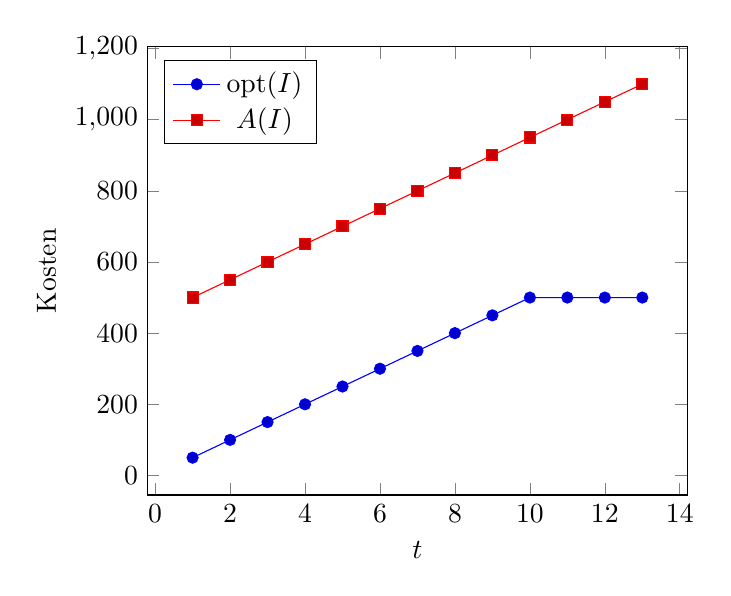
\begin{tikzpicture}
  \begin{axis}[ 
    xlabel=$t$,
    ylabel={Kosten},
	legend pos=north west
  ] 
    \addplot coordinates {
		(1,50)
		(2,100)
		(3,150)
		(4,200)
		(5,250)
		(6,300)
		(7,350)
		(8,400)
		(9,450)
		(10,500)
		(11,500)
		(12,500)
		(13,500)
	};
	\addlegendentry{$\operatorname{opt}(I)$}
    \addplot coordinates {
		(1,500)
		(2,550)
		(3,600)
		(4,650)
		(5,700)
		(6,750)
		(7,800)
		(8,850)
		(9,900)
		(10,950)
		(11,1000)
		(12,1050)
		(13,1100)
	};
	\addlegendentry{$A(I)$}
  \end{axis}
\end{tikzpicture}
\end{center}
\end{figure}

\begin{figure}
\caption{Verlauf der Competitive Ratio für SkiRental}
\label{fig.skirental.c}
\begin{center}
\begin{tikzpicture}
  \begin{axis}[ 
    xlabel=$t$,
    ylabel={$c(t)$},
	legend pos=north west
  ] 
    \addplot coordinates {
		(1,10)
		(2,5.5)
		(3,4)
		(4,3.25)
		(5,2.8)
		(6,2.5)
		(7,2.2857142857)
		(8,2.125)
		(9,2)
		(10,1.9)
		(11,2)
		(12,2.1)
		(13,2.2)
	};
  \end{axis}
\end{tikzpicture}
\end{center}
\end{figure}

Allgemein kann die Competitive Ratio für dieses Problem (mit allgemeinen Kosten $b$ für den Kauf bzw. $r$ für die Miete) beschrieben werden als
\[
	c_t = \begin{cases}
		\frac{b+(t-1)\cdot r}{t\cdot r}, & \text{wenn } r\cdot t \le b \\
		\frac{b+(t-1)\cdot r}{b}, & \text{sonst}
	\end{cases}
\]

\section{Zelluläre Automaten}

\begin{quote}Ein zellulärer Automat ist eine regelmäßige Annordnung von Zellen. Jede Zelle kann eine endliche Zahl
von Werten / Zuständen annehmen und hat eine begrenzte Zahl von Nachbarzellen, die sie beeinflussen
können. Das Muster des gesamten zellulären Automaten ändert sich in einzelnen Schritten, die durch eine
Reihe von Übergangsregeln bestimmt werden, die für alle Zellen gelten.\cite{beckmann}\end{quote}

Also:

\begin{definition}[Zellulärer Automat] Ein zellulärer Automat ist durch folgende Eigenschaften festgelegt:
\begin{itemize}
\item einen Zellularraum $R$,
\item eine endliche Nachbarschaft $N$, wobei $\forall r \in R \left(N_r \subset R\right)$,
\item eine Zustandsmenge $Q$,
\item eine Überführungsfunktion $\delta: Q^{|N| + 1}\mapsto Q$.
\end{itemize}
Die Zustandsübergänge erfolgen für alle Zellen nach derselben Überführungsfunktion und gleichzeitig. Die Zellzustände können wie die Zeitschritte diskret sein. \cite{wiki:zellautomat}

\end{definition}

\begin{bemerkung}
Aus dieser Definition folgt unmittelbar, dass der neue Zustand einer Zelle nur vom momentanen Zustand dieser Zelle sowie den Zuständen der Nachbarzellen abhängig sein kann.
\end{bemerkung}

Für zweidimensional organisierte $R$ sind zwei Arten von Nachbarschaft üblich:
\begin{description}
\item[Von-Neumann-Nachbarschaft] Die Nachbarschaft besteht jeweils aus den vier geographisch nächsten Nachbarzellen: $N_{i,j} = \left\{ R_{i,j-1}, R_{i,j+1}, R_{i-1,j}, R_{i+1,j}\right\}$
\item[Moore-Nachbarschaft] Die Nachbarschaft besteht jeweils aus allen Zellen der Von-Neumann-Nachbarschaft sowie zusätzlich der diagonalen Nachbarzellen:

$N_{i,j} = \left\{ R_{i,j-1}, R_{i,j+1}, R_{i-1,j}, R_{i+1,j},R_{i-1,j-1}, R_{i-1,j+1}, R_{i-1,j+1}, R_{i+1,j+1} \right\}$ \cite{schurr}
\end{description}

\begin{beisp}[Wolfram's eindimensionales Universum] Stephen Wolfram\footnote{Stephen Wolfram (* 29. August 1959), britischer Physiker und Mathematiker, Schöpfer der Software Mathematica sowie der Suchmaschine Wolfram Alpha \cite{wiki:wolfram}} definiert in \cite{wolfram2002} und in etlichen Arbeiten aus der Mitte der 1980er-Jahre einen parametrierbaren zellulären Automaten, der nur aus einer einzigen Raumdimension besteht\cite{wiki:wolfram}. In seiner einfachsten Ausprägung ist die Nachbarschaft $N_i$ definiert als $\left\{ R_{i-1}, R_{i+1} \right\}$, und jede Zelle kann genau zwei Zustände annehmen (tot und lebendig bzw. $0$ und $1$). Damit ist
\begin{equation*}
\delta : \left\{0,1\right\}^{|\left\{ R_{i-1}, R_{i+1}\right\}|+ 1} \mapsto \left\{0,1\right\} = \left\{0,1\right\}^3 \mapsto \left\{0,1\right\},
\end{equation*}
ergo existieren 8 mögliche Zustandsänderungen. Ein Beispiel:

\begin{table}[here]
\begin{center}
\begin{tabular}{|r||c|c|c|c|c|c|c|c|}
\hline
alte $R_{i-1}R_iR_{i+1}$ &111& 110 & 101 &100 &011 &010 &001 &000  \\\hline
neues $R_i$ & 0 & 1 & 1 & 0& 1 & 1 & 1 & 0 \\\hline
\end{tabular}
\end{center}
\caption{Wolfram-Konfiguration 110}
\label{wolfram110}
\end{table}

Man stellt nun fest, dass bei 8 möglichen Zustandsänderungen für die Anzahl der möglichen Konfigurationen gilt:
\begin{equation*}
|K| = |Q|^{|\operatorname{dom}(\delta)|} = 2^8 = 256.
\end{equation*}
Jeder dieser Konfigurationen kann eine natürliche Zahl $\left\{0, 1, 2, \dots, 255\right\}$ zugeordnet werden, indem die neuen $R_i$ wie oben tabelliert und pro Zeile als binäre Zahl aufgefasst werden \cite{betz2003}:

\begin{table}[here]
\begin{center}
\begin{tabular}{|c|c|c|c|c|c|c|c||l|}
\hline
111 & 110 & 101 &100 &011 &010 &001 &000 & Zahl \\\hline\hline
 0 & 0 & 0 & 0& 0 & 0 & 0 & 0 & $00000000_b = 0_d$ \\\hline
 0 & 0 & 0 & 0& 0 & 0 & 0 & 1 & $00000001_b = 1_d$ \\\hline
 0 & 0 & 0 & 0& 0 & 0 & 1 & 0 & $00000010_b = 2_d$ \\\hline
\multicolumn{9}{|c|}{$\vdots$} \\\hline
 0 & 1 & 1 & 0& 1 & 1 & 1 & 0 & $01101110_b = 110_d$ \\\hline
\multicolumn{9}{|c|}{$\vdots$} \\\hline
 1 & 1 & 1 & 1& 1 & 1 & 1 & 1 & $11111111_b = 255_d$ \\\hline
\end{tabular}
\end{center}
\caption{Alle Wolfram-Konfigurationen}
\label{wolframalle}
\end{table}

Dadurch ist es möglich, sämtliche eindimensionalen Wolfram-Universen durch eine einzige Zahl zu identifizieren.

Als besonders spannend hat sich die in Tabelle \ref{wolfram110} dargestellte Konfiguration 110 erwiesen, weil sie die Eigenschaft hat, ein Turing-vollständiges System zu sein \cite{betz2003, wolfram2002}. Dadurch ist sie die Konfiguration einer universellen Turingmaschine, die mit nur 2 Zuständen und 5 Symbolen umgesetzt werden kann -- somit hat die Wolfram-Konfiguration 110 als Turingmaschine einen Umfang von $2\cdot 5 = 10$ und zählt damit zu den kleinsten bis dato bekannten Turingmaschinen \cite{betz2003}.

\end{beisp}

\begin{beisp}[Game of Life]

\newcommand{\ql}{q_\textrm{lebend}}
\newcommand{\qt}{q_\textrm{tot}}

Das von Conway\footnote{John Horton Conway (* 26. Dezember 1937), englischer Mathematiker\cite{wiki:conway}} 1970 entworfene Game of Life ist eine bis heute populäre Umsetzung der Automatentheorie und insbesondere der Idee der zellulären Automaten \cite{wiki:gameoflife}.

Der ursprüngliche Entwurf befindet sich in einem zweidimensionalen $R$ unter Verwendung der Moore-Nachbarschaft. Die Zellen können zwei mögliche Zustände $\left\{\ql, \qt \right\}$ annehmen, und die Übergangsfunktion ist definiert \cite{Hafner} als:
\begin{equation*}
\delta(r, N) = \begin{cases}
\ql & (r = \qt \land \varsigma(\ql,N) = 3) \\
\qt & (r = \ql \land \varsigma(\ql, N) < 2) \\
\ql & (r = \ql \land 2 \leq \varsigma(\ql, N) \leq 3) \\
\qt & (r = \ql \land  \varsigma(\ql, N) > 3) \\
\qt & (\textrm{sonst})
\end{cases}
\end{equation*}
unter Zuhilfenahme der Statuszählfunktion
\begin{equation*}
\varsigma(q, N) = \sum\limits_{i=1}^8  \begin{cases} 1 & (N_i = q) \\ 0 & (N_i \neq q) \end{cases}
\end{equation*}

\end{beisp}

\section{Vom zellulären Automaten zur Differentialgleichung}

Die Berechnung und Darstellung physikalischer Begebenheiten (allgemein ausgedrückt durch folgende partielle Differentialgleichung, mit $u: u(\vec{x}, t)$)
\begin{equation*}
k_n \frac{\partial^n u}{\partial t^n} + k_{n-1} \frac{\partial^{n-1} u}{\partial t^{n-1}} + \cdots + k_1 \frac{\partial u}{\partial t} + k_0 = \frac{\partial^n u}{\partial  \vec{x}^n} + \frac{\partial^{n-1}}{\partial \vec{x}^{n-1}} + \cdots + \frac{\partial u}{\partial \vec{x}}
\end{equation*}
mit zellulären Automaten kann durchgeführt werden, indem folgendes getan wird:
\begin{itemize}
\item $R$ entspricht einer sinnvollen (groben) Diskretisierung der örtlichen Variablen $\vec{x}$ in einer, zwei oder drei Dimensionen
\item Jede Zelle in $R$ ist ein Tupel $(Q, D)$ mit $Q$ als einer Menge von berechnungsfernen Zustandsinformationen und den Differentialen nach der Zeit
\[
D = \left( u, \frac{\partial u}{t}, \frac{\partial^2 u}{\partial t^2}, \cdots, \frac{\partial^n u}{t^n} \right)  \in \mathbb{R}^n
\]
\item Eine neue Generation entspricht jeweils der fortgelaufenen Zeit $\partial t$, welche sehr fein diskretisiert werden muss
\item In der Übergangsfunktion $\delta$ steckt die eigentliche Differentialgleichung. In der Regel verändert sie nur die Elemente von $D$. Sollte die Differentialgleichung Terme mit verschiedenen Ordnungen enthalten, wird die Gleichung unter Zuhilfenahme entsprechender Hilfsgleichungen $\lambda_1, \lambda_2, \dots, \lambda_n$ in ein äquivalentes System gewöhnlicher Differentialgleichungen umgeformt. 
\end{itemize}

\section{Numerische Lösung von Differentialgleichungen}

Damit die numerische Lösung von Differentialgleichungen gelingt, sind vor allem zwei Fertigkeiten vonnöten: Die numerische Differenzierung sowie die numerische Integration. Wir wollen beide Gebiete kurz streifen, und zwar unter den für uns nützlichen Gesichtspunkten bezüglich der Wahl der Variablen sowie der vorliegenden impliziten Funktionen (beziehungsweise diskreten Werten als Zellinhalte des zellulären Automaten).

\subsection{Differenzierung nach dem Ort}

%Wir starten mit der homogenen Wellengleichung
%\begin{equation*}
%\frac{\partial^2 u}{\partial t^2} = k\cdot \frac{\partial^2 u}{\partial \vec{x}^2}
%\end{equation*}

Wir starten mit den gegebenen Werten $u_{\vec x}$ (den Zuständen der Zellen aus $R$). Daraus erhalten wir die diskrete Funktion
\[
u: R \mapsto \mathbb{R}, u(\vec x) = u_{\vec x}
\]

welche durch komponentenweises Einsetzen des Differenzenquotienten $\frac {\Delta u}{\Delta \vec x}$ folgendermassen differenzierbar ist (unter Zuhilfenahme des Einheitsvektors $\vec e_i$ für jede Komponente von $\vec x$ sowie der Erkenntnis, dass durch die diskrete Ausgangsfunktion $\Delta \vec{x}$ komponentenweise $1$ ist; die Interpretation, wo genau sich die Nachbarzelle $\vec x \pm n\cdot\vec e$ befindet, überlassen wir der für den zellulären Automaten gültigen Nachbarschaftsfunktion):
\begin{equation}\label{diffone}
	\left(\frac {\Delta}{\Delta \vec x} u\right)_{\vec x} = u_{\vec x} - \sum\limits_{i=1}^{\dim(\vec x)} u_{\vec x - \vec e_i}
\end{equation}
Diese Differenzen können natürlich wiederum differenziert werden:
\begin{eqnarray*}
	\left(\frac{\Delta}{\Delta \vec x}\left( \frac {\Delta}{\Delta \vec x} u \right)_{\vec x}\right)_{\vec x} &=& \left(\frac {\Delta}{\Delta \vec x} u\right)_{\vec x} - \sum\limits_{i=1}^{\dim(\vec x)} \left( \frac {\Delta}{\Delta \vec x} u \right)_{\vec x - \vec e_i}
\end{eqnarray*}
Durch Einsetzen von \ref{diffone} in die obige Gleichung ergibt sich dann für die Differenz zweiter Ordnung:
\begin{eqnarray*}
\left( \frac{\Delta^2}{\Delta \vec x^2} u\right)_{\vec x} &=& u_{\vec x} - \sum\limits_{i=1}^{\dim(\vec x)} u_{\vec x - \vec e_i} - 
\sum\limits_{i=1}^{\dim(\vec x)} \left( u_{\vec {x^*}} - \sum\limits_{i=1}^{\dim(\vec x)} u_{\vec {x^*} - \vec e_i} \right)_{\vec {x^*} := \vec x - \vec e_i} \\
&=& u_{\vec x} - \sum\limits_{i=1}^{\dim(\vec x)} u_{\vec x - \vec e_i} - \sum\limits_{i=1}^{\dim(\vec x)} u_{\vec x - \vec e_i} + \sum\limits_{i=1}^{\dim(\vec x)} u_{\vec x - 2\vec e_i} \\
&=&  u_{\vec x} - 2\cdot\sum\limits_{i=1}^{\dim(\vec x)} u_{\vec x - \vec e_i} + \sum\limits_{i=1}^{\dim(\vec x)} u_{\vec x - 2\vec e_i}
\end{eqnarray*}

\begin{bemerkung}[Indizes]
Da der Definitionsbereich der besprochenen Funktion diskret ist, verringert sich die Kardinalität des Definitionsbereichs der Differenzen mit fortschreitender Ordnung jeweils um $1$ pro Dimension. Geographisch gesprochen, liegt die Differenz zweier Zellen ja eigentlich auf der gemeinsamen Kante dieser zwei Zellen. Daher ist es in der Praxis sinnvoll, die Differenzen gerader Ordnungen (bei deren Berechnung wie eben gesehen 3 Zellen pro Dimension involviert sind) jeweils in die Zelle in der Mitte zu schieben. Im Falle der zweiten Ordnung ergibt sich damit:
\begin{equation}
\left( \frac{\Delta^2}{\Delta \vec x^2} u\right)_{\vec x} =\sum\limits_{i=1}^{\dim(\vec x)} u_{\vec x - \vec e_i}  -2\cdot u_{\vec x} + \sum\limits_{i=1}^{\dim(\vec x)} u_{\vec x + \vec e_i}
\end{equation}
\end{bemerkung}

\subsection{Integration nach der Zeit mit Einschrittverfahren}

\newcommand{\intr}{\mathbf{int}}
\renewcommand{\d}{\mathrm{d}}
\newcommand{\duxt}{\left(\frac{\Delta}{\Delta \vec x}u \right)_{\vec x, t}}
\newcommand{\duxtp}[1]{\left(\frac{\Delta}{\Delta \vec x}u \right)_{\vec x, t + #1 h}}

\subsubsection{Forderung}

Wir starten mit den gegebenen Werten $\left(\frac{\Delta}{\Delta \vec x}u \right)_{\vec x}$ (den vorgängig berechneten Differenzen zwischen den Zellen). Wir definieren die allgemeine Integrationsfunktion
\[
\intr :  \mathbb{R}^2 \mapsto \mathbb{R}
\]
für welche jeweils gelten muss:
\[
\intr\left(\duxt, h \right) \approx \int\limits_t^{t+h} u_{\vec x} \d t
\]

Da die $u_{\vec x}$ zu jedem Zeitpunkt $t$ (also pro Zeitschritt $h$ beziehungsweise $\d t$) jeweils von ihren Nachbarzellen abhängen, ist es vonnöten, sämtliche Zellen für einen einzigen Zeitschritt simultan durchzurechnen.

\subsubsection{Die impliziten Runge-Kutta-Verfahren}

Da uns hier nur Einschrittverfahren interessieren, schauen wir uns im Detail die Klasse der Runge-Kutta-Verfahren\footnote{Carl David Tolmé Runge (1856--1927), deutscher Mathematiker \cite{wiki:Runge}}\footnote{Martin Wilhelm Kutta (1867--1944), deutscher Mathematiker \cite{wiki:Kutta}} an, welche auf dem expliziten Euler-Verfahren\footnote{Leonhard Euler (1707--1783), Schweizer Mathematiker und Physiker \cite{wiki:Euler}} basieren und durch Butcher-Tableaux\footnote{John Charles Butcher (*1933), neuseeländischer Mathematiker \cite{wiki:Butcher}} allgemein definiert werden können.

Sämtliche Runge-Kutta-Verfahren können folgendermassen dargestellt werden:
\[
y_{n+1} = y_n + h\cdot \sum\limits_{j=1}^s \gamma_j \cdot k_j
\]
wobei $h$ die gewählte Schrittweite, $\gamma_j$ die charakteristischen Koeffizienten des gewählten Verfahrens sowie $k_j$ die Auswertungen der zu integrierenden Funktion $f$ an bestimmten Stützstellen repräsentieren. Für $k_j$ gilt dann:
\[
k_j = f\left(t_n + h\cdot\alpha_j, y^n + h\cdot \sum\limits_{i=1}^m \beta_{j,i}\cdot k_i \right)
\]

wobei $\alpha_j$ sowie $\beta_{j,i}$ wiederum charakteristische Koeffizienten sind \cite{Massjung, wiki:RungeKutta}, welche zusammen mit den $\gamma_j$ in einem Butcher-Tableau folgendermassen angeordnet werden können:
\[
\begin{bmatrix}
\begin{array}{c|c}
a & B\\
\hline     & c \\
\end{array}
\end{bmatrix} = \begin{bmatrix}
\begin{array}{c|cccc}
  \alpha_1    & \beta_{1,1} & \beta_{1,2}& \cdots & \beta_{1,m}\\
  \alpha_2    & \beta_{2,1} & \beta_{2,2}& \cdots & \beta_{2,m}\\
  \vdots & \vdots & \vdots& \ddots& \vdots\\
  \alpha_m    & \beta_{m,1} & \beta_{m,2}& \cdots & \beta_{m,m}\\
  \hline & \gamma_1    & \gamma_2   & \cdots & \gamma_m\\
\end{array}

\end{bmatrix}
\]

Runge-Kutta-Verfahren sind im Allgemeinen implizit, weil zur Bestimmung der $k_j$ sowie $y^{n+1}$ ein (mindestens lineares) $(m+1)\times(m+1)$-Gleichungssystem gelöst werden muss; dies verursacht natürlich entsprechende Kalamitäten. Solchartige Verfahren sind aber sehr stabil.\cite{Deuflhard}

\subsubsection{Die expliziten Runge-Kutta-Verfahren}

Ist es nun möglich, Koeffizienten zu finden, deren Matrix $B$ strikte nilpotente untere Dreiecksgestalt hat, so spricht man von einem expliziten Verfahren, weil sich das Gleichungssystem einfach durch Rückwärtseinsetzen lösen lässt (sogar wenn es nichtlinear ist):

\[
\begin{bmatrix}
\begin{array}{c|c}
a & B\\
\hline     & c \\
\end{array}
\end{bmatrix} = \begin{bmatrix}
\begin{array}{c|cccc}
  \alpha_1 & 0  \\
  \alpha_2    & \beta_{2,1} & 0\\
  \vdots & \vdots & \vdots& \ddots\\
  \alpha_m    & \beta_{m,1} & \beta_{m,2}& \cdots & 0\\
  \hline & \gamma_1    & \gamma_2   & \cdots & \gamma_m\\
\end{array}

\end{bmatrix}
\]

Für ausgewählte explizite Verfahren lassen sich nun sowohl Butcher-Tableau als auch die geforderte Integrationsfunktion $\intr$ folgendermassen aufstellen:

\begin{description}
\item[Euler]
\begin{eqnarray*}
\begin{bmatrix}
\begin{array}{c|c}
a & B\\
\hline     & c \\
\end{array}
\end{bmatrix}
 &=& \begin{bmatrix}
\begin{array}{c|c}
0 & 0 \\\hline
& 1
\end{array}
\end{bmatrix} \\
\Rightarrow \intr\left(\duxt, h\right) &=& u_{\vec x, t} + h\cdot \duxt
\end{eqnarray*}

\item[Runge-Kutta 2. Ordnung]
\begin{eqnarray*}
\begin{bmatrix}
\begin{array}{c|c}
a & B\\
\hline     & c \\
\end{array}
\end{bmatrix} &=& \begin{bmatrix}
\begin{array}{c|cc}
0 & 0 \\
\frac 1 2 & \frac 1 2 & 0 \\\hline
& 0 & 1
\end{array}
\end{bmatrix} \\
\Rightarrow \intr\left(\duxt, h\right) &=& u_{\vec x, t} + h\cdot k_2 \\
%k_2 &=& \left(\frac{\Delta}{\Delta t} u \right)_{\vec x, t + \frac 1 2 h} \\
%&=&  u_{\vec x, t} + h\cdot\intr\left(\duxtp{\frac 1 2} \right) \\
&=&  u_{\vec x, t} + h\cdot\intr\left(\duxtp{\frac 1 2} \right) \\
\end{eqnarray*}

\end{description}

\subsection{Die homogene Wellengleichung}

Am Beispiel der homogenen Wellengleichung soll nun die Umsetzung einer Differentialgleichung in einem zellulären Automaten gezeigt werden. Die homogene Wellengleichung ist eine partielle Differentialgleichung zweiter Ordnung und lautet \cite{wiki:Wellengleichung}:
\[
\frac 1 {c^2} \frac{\partial^2 u}{\partial t^2}-\sum_{i=1}^{n} \left( \frac{\partial^2 u}{\partial x_i^2} \right)  = 0
\]

oder ein bisschen umgeformt ($\frac 1 {c^2} = \frac 1 k$) und die Einzelkomponenten $x_1, x_2, \dots, x_n$ als Vektor geschrieben:
\[
\frac {\partial^2 u} {\partial \vec x^2} = k \cdot \frac {\partial^2 u}{\partial t^2}
\]

Nach diesem Schema soll zweimal nach dem Ort differenziert und zweimal nach der Zeit integriert werden:

%\begin{equation*}
%\begin{array}{rcl}
\begin{align*}
u_i &&& u_i(t+\Delta t) = u_i(t) +  \frac{\partial u_i(t+\Delta t)}{\partial t}\Delta t \\
\downarrow &&& \uparrow \\
\frac{\partial u_i}{\partial \vec x} = u_i - \sum u_{i-1} &&& \frac{\partial u_i(t+\Delta t)}{\partial t} = \frac{\partial u_i(t)}{\partial t} + \frac{\partial^2 u}{\partial t^2}\Delta t \\
\downarrow &&& \uparrow \\
\frac{\partial^2 u_i}{\partial \vec x^2} = -2u_i + \sum u_{i-1} + \sum u_{i+1} & \underbrace{\longrightarrow}_{\frac{\partial^2 u}{\partial t^2} = k\cdot \frac{\partial^2 u}{\partial \vec{x}^2}} && \frac{\partial^2 u}{\partial t^2}
\end{align*}
%\end{array}
%\end{equation*}

Als Nachbarschaft wird die Von-Neumann-Nachbarschaft gewählt, weil bei der Moore-Nachbarschaft die Eckzellen nicht linear unabhängig wären. Ergo ergibt sich folgende Übergangsfunktion $\delta$, abhängig von der Zelle $r$ sowie den Nachbarzellen $n, e, s, w$ (Norden, Osten, Süden, Westen für ein zweidimensionales Zellfeld):

\begin{eqnarray*}
\delta(r, n, e, s, w) &=& \begin{bmatrix}
	\delta_{\frac {\Delta r}{\Delta t}}(r,n,e,s,w) \\
	\delta_{\frac {\Delta^2 r}{\Delta t^2}}(r,n,e,s,w)
\end{bmatrix} \\
&=& \begin{bmatrix}
	r_{\frac {\Delta r}{\Delta t}} + \delta_{\frac {\Delta^2 r}{\Delta t^2}}(r,n,e,s,w)  \cdot \Delta t \\
	\frac{\Delta^2 r}{\Delta \vec x^2} \cdot k  \\
\end{bmatrix} \\
&=& \begin{bmatrix}
	r_{\frac {\Delta r}{\Delta t}} + \delta_{\frac {\Delta^2 r}{\Delta t^2}}(r,n,e,s,w)  \cdot \Delta t \\
	(-2 r + \frac 1 2 (n + e + s + w)) \cdot k
\end{bmatrix}
\end{eqnarray*}

Und damit sind wir im Grunde bereit für die Implementation.

\chapter{Bemerkungen zur Implementation}

\section{Wahl des Umfelds}

Die Wahl des Umfelds fiel auf eine Kombination aus JavaScript und dem HTML5-{\tt canvas}-Element für die grafische Ausgabe. Die hauptsächlichen Gründe dafür sind die einfache Umsetzung sowie die sehr gute Portabilität, vorallem auch auf portable Devices mit Touch-Bedienung. Dadurch kommt der primäre Use Case der Software (Bewegung einer Flüssigkeit mittels dem Pointing Input) besonders gut zur Geltung, weil der Input eben mit dem Finger vorgenommen werden kann.

Bedenken wurden vorgängig und während der ersten Implementierungsphase vor allem in Bezug auf die Perfomance geäussert, konnten aber im Laufe des Projekts zerstreut werden, auch weil gezeigt werden konnte, dass Optimierungen möglich sind (paralleles Berechnen, Umstellung von Vektorgrafik-Operationen auf Bitmap-Manipulationen).

Als Alternativen waren das Game-Framework XNA sowie die 3D-LED-Installation in der Haupthalle des Zürcher Hauptbahnhofs in Betracht gezogen worden.

\section{Implementatorische Paradigmen}

Da JavaScript keine typisierte Sprache ist, ist ein formaler Aufbau à la Java weder möglich noch sinnvoll. Wir lehnen uns in unserem Stil dem Duck-Typing-Paradigma von Ruby an, damit sind wir inhärent polymorph. Die in den in den folgenden Abschnitten dargestellten UML-Diagrammen vorkommenden abstrakten Klassen oder Interfaces existieren darum nicht im realen Code, sondern dienen mehr der Veranschaulichung und Strukturierung der Diagramme.

Natürlich gibt es keine Regel ohne Ausnahme: Die Klasse {\tt ATusk} existiert tatsächlich und wird über Prototyping gesubklasst -- einfach damit wir das mal gemacht haben \cite{OOJSone, OOJStwo, OOJSthree}.

\section{Architektur}

Eine Übersicht über die grobe Architektur sei hier als Package-Diagramm skizziert:

%\includegraphics[scale=0.7]{uml/Architektur.pdf}

\section{Testing}

Unit Testing mit JavaScript ist nicht ganz einfach -- aber möglich und natürlich sinnvoll. Wenn die Unit Tests in einem tatsächlichen Browser auszuführen sind, weil sie beispielsweise mit dem Document Object Model interagieren, führt das zwangsläufig zu Mühsamitäten, vor allem bezüglich Continuous Integration.

Da allerdings das UI nur einen kleinen Teil unseres Programms ausmacht, schien es ratsam, vor allem die anderen Bereiche zu testen. Daraus ergibt sich die Möglichkeit, auf eine Implementation von JavaScript in einem nicht-interaktiven Kontext zu setzen. Die Wahl fiel auf Node.js, eine auf WebKit aufbauende Server-Implementation von JavaScript \cite{Node}, sowie das Test-Framework Mocha \cite{Mocha}.
Da das produktive Programm eine reine Browser-Geschichte ist, stehen während des produktiven Betriebs weder Build-Tools noch Server zur Verfügung, alle JavaScript-Files werden vom verwendenden HTML-Dokument über profane {\tt <script>}-Tags eingebunden.
Um das sich daraus ergebende Dilemma zwischen Test- und Produktionsumgebung zu lösen, werden die Komponenten über Node-Module wo nötig zusammengestöpselt, aber nur dann, wenn Node tatsächlich zur Verfügung steht (der Ausführer also ein Test Runner ist):

\begin{lstlisting}
if (typeof(module) != "undefined") {
	module.exports = CellularAutomata;
	var Cell = require('../../src/automata/Cell.js');
	var Swimmer = require('../../src/automata/Swimmer.js');
}
\end{lstlisting}

Ein Unit Test (unter Verwendung der Should-Assertion Library) sieht dann beispielsweise folgendermassen aus:

\begin{lstlisting}
describe('CellularAutomata', function() {

	it('should step without Tusk', function() {
		var auto = new CellularAutomata();
		auto.initCells();
		var iterations = auto.iterations;
		auto.step();
		auto.iterations.should.equal(iterations+1);
	});

});
\end{lstlisting}

Die Summe der Tests kann dann auf der Kommandozeile (oder durch einen CI-Server) aufgerufen werden mit:
\begin{verbatim}
~/node node_modules/mocha/bin/mocha
\end{verbatim}

\section{Automata}

Die Klasse {\tt CellularAutomata} implementiert zusammen mit ihren Hilfsklassen den zellulären Automaten:

%\includegraphics[scale=0.7]{uml/Automata.pdf}

{\tt CellularAutomata} definiert zuallererst einmal eine coole Hilfsmethode, welche über alle Zellen des Automaten iteriert und eine beliebige Funktion ausführt:

\begin{lstlisting}
this.forEachCell = function(fn) {
	for (var x = 0; x < this.cols; x++) {
		for (var y = 0; y < this.rows; y++) {
			var cell = this.model[x][y];
			fn(cell);
		}
	}
};
\end{lstlisting}

Diese Methode wird dann beispielsweise während der Initialisierung der Zellen folgendermassen verwendet\footnote{Ein Wort zu der auf den ersten Blick unnötig komplizierten Definition der von {\tt this.forEachCell()} auszuführenden anonymen Funktion: In JavaScript wird der Scope von Variablen durch die Funktion und nicht den Block begrenzt, darum gilt als Best Practice zur expliziten Scope-Gebung im Allgemeinen das Wrappen in einer anonymen Funktion und unmittelbarer Ausführung derselben \cite{UnderstandingClosures}. Da {\tt this} schlussendlich auch nur eine Variable in einem Funktionsscope ist, wäre {\tt this.tusk} keine sinnvolle Referenz, weil {\tt this} nicht bedingungslos (wie in anderen funktionalen Programmiersprachen üblich) eine Instanz von {\tt CellularAutomata} (den Definitionsscope von {\tt wireNeighbourCells()}), sondern der Caller ist (falls das Drücken eines Buttons zu einem Aufruf von {\tt wireNeighbourCells()} führte, wäre {\tt this} das Browser-{\tt document}).}:
\begin{lstlisting}
this.wireNeighbourCells = function() {
	if (this.tusk != null) {
		this.forEachCell(
			(function(automata) {
				return function(cell) {
					cell.neighbours = automata.tusk.getNeighbours(cell, automata.model);
				};
			})(this)
		);
	}
}
\end{lstlisting}

Des weiteren führt {\tt CellularAutomata} die Zelltransitionen durch:

\begin{lstlisting}
this.step = function() {		
	if (this.tusk != null) {
		this.fireEvents();		
		this.integration.integrate(this);
		this.travelSwimmers();
	}	
	this.iterations++;	
}
\end{lstlisting}

Spannend hierbei zu sehen ist die Aufteilung der Verantwortlichkeiten. {\tt CellularAutomata} kennt weder  die Übergangsfunktion $\delta$, die Nachbarschaftsfunktion\footnote{Wie im Listing weiter oben ersichtlich, werden sämtliche Nachbarzellen sämtlicher Zellen während der Initialisierung aufgefunden und verknüpft. Da sich gemäss der Definition des Zellulären Automaten die Nachbarschaftsbeziehungen zwischen Zellen nie ändern, ergo von Anfang an feststehen, ist dies eine zulässige Performance-Optimierung; ansonsten müsste auf das Feld der Zellen bei jedem Iterationsschritt mindestens $|R|\cdot |N|$ mal zugegriffen werden (wobei $R$ der ganze Zellraum und $N$ die Menge der Nachbarzellen einer Zelle ist).} noch die Integrationsfunktion $\intr$, sondern verwendet via Strategy-Pattern die ihr zugeteilten Implementationen (beispielsweise die Wellengleichung mit dem Euler-Verfahren).

Es ist sogar so, dass der eigentliche Zellinhalt (der ja nur von der Übergangsfunktion $\delta$ verwendet wird) unbekannt ist. Jeder Tusk besitzt entsprechend eine Factory-Methode, um einen solchen Zellinhalt herzustellen. Die Unterschiede in den Datenstrukturen sind frappant. Das Game Of Life begnügt sich mit:

\begin{lstlisting}
this.createCellData = function() {
	return {status: 0};
}
\end{lstlisting}

wogegen die Wellengleichung einige Daten mehr benötigt:
\begin{lstlisting}
this.createCellData = function() {
	return {
		u: 0,
		udx: 0,
		udxdx: 0,
		udtdt: 0,
		udt: 0,
		vx: 0,
		vy: 0
	};
};
\end{lstlisting}

\section{Integration}

Die Wahl der Integrationsmethode ist wiederum eine Anwendung des Strategy-Patterns, wie in der Übersicht skizziert:

%\includegraphics[scale=0.7]{uml/Integration.pdf}

{\tt integrate()} iteriert dann typischerweise über alle Zellen des Automaten und führt die Integration unter ein- oder mehrmaligem Aufruf der Übergangsfunktion $\delta$ des Tusk durch. Hier ist das Beispiel für das explizite Euler-Verfahren dargestellt:

\begin{lstlisting}
this.integrate = function(automata) {
	var dt = 1 / automata.tusk.slices;
	for (var t = 0; t < automata.tusk.slices; t++) {
		
		automata.forEachCell(
			function(cell) {
				var differentials = automata.tusk.calcDifferentials(cell, dt, function(cell2) {
					return cell2.currentData;
				});
				cell.nextData = automata.tusk.applyDifferentials(cell, dt, differentials, function(cell2) {
					return cell2.currentData;
				})
			}
		);
		
		automata.forEachCell(
			function(cell) {
				cell.currentData = cell.nextData;
			}
		);
		
	}
}
\end{lstlisting}


\section{Tusks, Regen, Enten und andere obskure Objekte}

Die Tusks sind die Hard Worker in der ganzen Konstruktion:

%\includegraphics[scale=0.7]{uml/Tusk.pdf}

\subsection{Zellzustände und Pools}

Der Aufbau der Zellstände sind nur für den Tusk von Bedeutung; die Verwender des Tusk (beispielsweise {\tt CellularAutomata} weiss nichts darüber. Der Tusk implementiert die $\delta$-Funktion (über {\tt calcDifferentials()} und {\tt applyDifferentials()}) und dient als Fassade für alle weiteren Zellzustands-Operationen:

\begin{description}
\item[createCellData()] dient als Factory-Methode, um neue Zellzustände herzustellen;
\item[setCellValue(Cell, value)] setzt den $u$-Wert einer Zelle,
\item[getVelocity(Cell)] liefert den Geschwindigkeitsvektor einer Zelle (falls sinnvoll).
\end{description}

Des weiteren kann ein Tusk beliebig viele Pools definieren, die im Normalfall einen einzigen Aspekt des Zellzustands visualisieren sollen. Diese Pools können mit einem Namen und einem Bild versehen werden und tauchen dann in der Liste der Sekundär-Pools der View auf. Die Methode {\tt pool.getValue()} liefert dann den Wert dieses Aspektes, wie zum Beispiel das erste Differential $\frac{\Delta}{\Delta \vec x} u$ in {\tt DifferentialEquation}:

\begin{lstlisting}
this.pools = [
	new Pool("du/dx", "_assets/pics/udx.png", function(cell) {
		return cell.currentData.dudx;
	})
];
\end{lstlisting}

Für den Primär-Pool für $u$ gilt dasselbe:
\begin{lstlisting}
this.primaryPool = new Pool("u", "", function(cell) {
	return cell.currentData.u; }
);
\end{lstlisting}

\subsection{Swimmers}

Zu einer ernstzunehmenden Simulation von Flüssigkeiten gehören natürlich schwimmende Objekte -- im Idealfall sind das Badeenten. Diese Badeenten bewegen sich entlang der Gefälle der Oberfläche, sprich der Ableitungsvektoren entlang der Dimensionen $\frac {\Delta}{\Delta x_1}u, \frac {\Delta}{\Delta x_2}u, \dots, \frac {\Delta}{\Delta x_n}u$. Aus diesem Grund gibt es im Tusk die Methode {\tt getVelocity(Cell)}, zum Beispiel für die Wellengleichung:

\begin{lstlisting}
this.getVelocity = function(cell) {
	var v = new Vector();
	v.x = cell.currentData.vx;
	v.y = cell.currentData.vy;
	return v;
}
\end{lstlisting}

Die Badeenten (oder auch Fussbälle) ändern dann ihre Positionen anhand dieser Vektoren:
\begin{lstlisting}
this.forEachSwimmer(
	(function(automata) {
		return function(swimmer) {
			var cell = automata.model[Math.floor(swimmer.location.y)][Math.floor(swimmer.location.x)];
			var velocity = automata.tusk.getVelocity(cell);
			swimmer.move(velocity);
		}
	})(this);
}

\end{lstlisting}

Zu guter Letzt wird noch der Darstellungswinkel der Schwimmer über ein paar Takte Trigonometrie (für zweidimensionale Zellräume) berechnet:
\[
\varphi = \begin{cases}
\tan^{-1} \left(-\frac x y\right) & \textrm{für } x \ge 0 \land y < 0, \\
\tan^{-1} \left(-\frac y x\right)  + \frac \pi 2& \textrm{für } x > 0 \land y \ge 0, \\
\tan^{-1} \left(-\frac x y\right)  + \pi& \textrm{für } x \le 0 \land y > 0, \\
\tan^{-1} \left(-\frac y x\right)  + \frac 3\pi 2& \textrm{für } x < 0 \land y \le 0
\end{cases}
\]

Die dritte Art von Schwimmern sind Boote (aus Holz), die über einen Motor verfügen und darum eine Eigengeschwindigkeit haben, die zur aus dem Gefälle resultierenden Geschwindigkeit gerechnet wird:

\begin{lstlisting}
function AutoSwimmer() {
	this.move = function(d) {
		this.velocity
			= this.autoVelocity.clone().scale(0.8).add(d.scale(0.2));
		this.location.add(this.autoVelocity);
	}
}
\end{lstlisting}

\subsection{Events}

Events bringen die Natur zurück in die Informatik durch periodische Manipulation der Zellzustände. Die Tusks definieren, welche Events für sie sinnvoll sind. Hier die Übersicht:

%\includegraphics[scale=0.7]{uml/Events.pdf}

{\tt CellularAutomata} lässt dann vor jeder Iteration jedes Event ausführen:

\begin{lstlisting}
this.fireEvents = function() {
	// fire events, such as rain, vorteces etc.
	if (this.tusk.events) {
		for (var i = 0; i < this.tusk.events.length; i++) {
			if (this.tusk.events[i].enabled) {
				this.tusk.events[i].apply(this);
			}
		}
	}
}
\end{lstlisting}

Wenn man beispielsweise Regen als gleichverteiltes Verändern der Wassermenge an einzelnen Punkten betrachtet, könnte man folgendes programmieren:

\begin{lstlisting}
function RainEvent(applyCell) {

	this.dropsPerIteration = 4;
	this.sign = 1;
	
	this.apply = function(automata) {
		var drops = this.dropsPerIteration == 0 ? 0
			: this.dropsPerIteration >= 1 ? this.dropsPerIteration
			: automata.iterations
				% (Math.floor(1 / this.dropsPerIteration)) == 0 ? 1 : 0;
		
		for (var i = 0; i < drops; i++) {
			var x = Math.floor(Math.random() * automata.cols);
			var y = Math.floor(Math.random() * automata.rows);
			var cell = automata.model[x][y];
			this.sign = this.sign * -1;
			applyCell(cell, this.sign);
		}
	}
}
\end{lstlisting}

Da die Tusks die Events definieren (in diesem Beispiel so:)

\begin{lstlisting}
this.events = [
	new RainEvent(
		function(cell, value) {
			cell.currentData.udt = value - cell.currentData.u;
			cell.currentData.u = value;
		}
	),
 	/* ... */
];
\end{lstlisting}

wissen die Events nichts von den Tusks, also geben die Tusks eine Funktion mit, mittels derer das Event die Zellzustände sinnvoll manipulieren kann ({\tt applyCell}).

Des weiteren ist jedes Event unter Umständen in Aspekten konfigurierbar -- im Beispiel des Regens die Intensität, dargestellt als Anzahl Tropfen pro Iteration. Die View weiss allerdings nichts davon, also braucht es hier eine Konstruktion, mit der das Event sein Konfigurations-UI dynamisch zur Verfügung stellen kann. Dies wird von der Methode {\tt createView()} übernommen:

\begin{lstlisting}
this.createView = function(doc) {
	var table = doc.createElement("table");
	var tr1 = doc.createElement("tr");
	var tr1Label = doc.createElement("td");
	var tr1Val = doc.createElement("td");
	var drops = doc.createElement("input");
	drops.type = "text";
	drops.style.width = "50px"
	drops.value = this.dropsPerIteration;
	drops.onchange = (function(evt, val) {
		return function() {
			evt.dropsPerIteration = val.value;
		}
	})(this, drops);
	
	table.appendChild(tr1);
	tr1.appendChild(tr1Label);
	tr1.appendChild(tr1Val);
	tr1Val.appendChild(drops);
	tr1Label.innerHTML = "Drops/Iteration";
	
	return table;
}
\end{lstlisting}

Sobald die View dann weiss, welcher Tusk aktiv ist (beispielsweise durch Auswahl durch den Benutzer), durchläuft die View alle Events des Tusks, ruft die entsprechende {\tt createView()}-Methode auf und baut das zurückgegebene Element ins {\tt document} ein.

\section{View}

Um auch das UI testbar zu halten, wird es hauptsächlich in eine {\tt View}- und eine {\tt Doc}-Klasse aufgeteilt, wovon die zweitere das HTML-{\tt document} abstrahiert und für das Testing entsprechend zu mocken ist:

%\includegraphics[scale=0.7]{uml/View.pdf}

Die für die Interaktivität nötige Logik ist in den verschiedenen Controller-Klassen, hier als Anschauung ein Ausschnitt aus {\tt TransportController}:

\begin{lstlisting}
function TransportController(doc, view) {
	
	this.doc = doc;
	this.view = view;
	
	this.running = false;

	/* ... */

	this.step = function() {
		this.view.automata.step();
		this.view.paintAll();
		this.doc.iterationLabel.innerHTML = this.view.automata.iterations;
		if (this.running) {
			window.setTimeout((function(controller) {
				return function() {
					controller.step();
				};
			})(this), 0);
		}
	}

	/* ... */

}
\end{lstlisting}

\subsection{Pool Canvas Painting}

Die grafische Ausgabe des zellulären Automaten findet in einem {\tt canvas}-Element statt, in das mittels JavaScript-Code gezeichnet wird. Es gibt verschiedene Arten, dies zu tun, ergo existieren verschiedene Implementationen:

%\includegraphics[scale=0.7]{uml/Painters.pdf}

Die relevanten Methoden sind:

\begin{description}
\item[\tt begin()] Beginnt den Zeichnungszyklus.
\item[\tt paintCell(cell)] Zeichnet eine einzelne Zelle ({\tt cell}) neu.
\item[\tt paintSwimmer(swimmer, cell)] Zeichnet eine Ente ({\tt duck}) in eine einzelne Zelle ({\tt cell}).
\item[\tt end()] Beendet den Zeichnungszyklus.
\end{description}

Die Methoden {\tt begin()} und {\tt end()} sind für Implementationen gedacht, die sich nur sinnvoll verhalten wenn sie den gesamten {\tt canvas} neu bezeichnen können und deswegen nach einem atomaren Aufruf von {\tt paintCell()} einen inkonsistenten Zustand aufweisen.

In den folgenden Abschnitten sind die verfügbaren Implementationen (ausser {\tt NoopCanvasPainter}, welche trivial ist und verwendet werden kann, um die grafische Ausgabe komplett abzuschalten) grob erklärt. 

\subsubsection{{\tt VectorCanvasPainter}}

Diese Klasse bezeichnet den {\tt canvas} durch Vektorgrafik-Operationen:

\begin{lstlisting}
this.paintCell = function(cell) {
	var x = cell.x * this.scaling.x;
	var y = cell.y * this.scaling.y;
	
	var baseColor = this.baseColor;
	var color = ViewUtils.getFormattedColor(this.pool.getValue(cell), baseColor.r, baseColor.g, baseColor.b);
	
	this.context.fillStyle = color;
	this.context.fillRect(x, y, this.scaling.x, this.scaling.y);
};
\end{lstlisting}

\subsubsection{{\tt PixelCanvasPainter}}

Diese Klasse bezeichnet den {\tt canvas} durch direkte Pixel-Manipulationen. Grundsätzlich funktionert das folgendermassen \cite{mdn:PixelCanvasDoku}:

\begin{lstlisting}
var myImageData = context.createImageData(cssWidth, cssHeight);
// ... do manipulation here ...
context.putImageData(myImageData, 0, 0);
\end{lstlisting}

Es muss allerdings gesagt werden, dass die Methode {\tt putImageData()} in allen verfügbaren Implementationen (Gecko, WebKit usw.) einigermassen langsam ist. Dies wird vor allem damit erklärt, dass das zu manipulierende Pixel-Array ({\tt myImageData.data} in unserem Beispiel) ein Array von Integern ist, das von {\tt putImageData()} jeweils noch durchlaufen und auf Gültigkeit (Werte $\in [0: 255]$) geprüft werden muss.

Andrew J. Baker zeigt nun in \cite{mdn:PixelCanvas} einen Weg, durch den die Pixelmanipulationen drastisch beschleunigt werden können (solange die verwendete Implementation den Typ {\tt Uint8ClampedArray} unterstützt, wie vom HTML5-Standard  \cite{wthree:twodcanvas} eigentlich vorgesehen).

Dazu ist es erst einmal nötig, in {\tt begin()} die Pixel-Daten vorzubereiten:

\begin{lstlisting}
this.begin = function() {
	this.imageData = this.context.createImageData(WIDTH, HEIGHT);
	this.buf = new ArrayBuffer(this.imageData.data.length);
	this.buf8 = new Uint8ClampedArray(this.buf);
	this.data = new Uint32Array(this.buf);
};
\end{lstlisting}

Dadurch ist es möglich, die in {\tt this.data} enthaltenen Daten als ganze Pixel zu bearbeiten (und nicht den Alpha-, Rot-, Grün- und Blau-Kanal einzeln):

\begin{lstlisting}
this.paintCell = function(cell) {
	var x = cell.x * this.scaling.x;
	var y = cell.y * this.scaling.y;
	
	var baseColor = this.baseColor;
	var color = ViewUtils.getColor(this.pool.getValue(cell), baseColor.r, baseColor.g, baseColor.b);
		
	for (var ix = x; ix < x + this.scaling.x; ix++) {
		for (var iy = y; iy < y + this.scaling.y; iy++) {
			var p = (iy * this.view.CANVAS_WIDTH + ix);
			
			this.data[p] =
				(255   << 24) | // alpha
				(color.b << 16) |
				(color.g <<  8) |
				color.r;
		}
	}
};
\end{lstlisting}

Abschliessend werden dann die manipulierten Pixel wieder zurückgeschrieben:

\begin{lstlisting}
this.end = function() {
	this.imageData.data.set(this.buf8);
	this.context.putImageData(this.imageData, 0, 0);
};
\end{lstlisting}

Ein Problem bleibt aber noch: By design exponiert {\tt Uint32Array} die exakten Daten so wie sie im Memory liegen -- das heisst, die obige Implementation funktioniert nur für Geräte, die mit Little Endian kutschieren. Bei der Ausführung auf Big Endian-Geräten würden die Farben ein bisschen lustig aussehen, weil die Werte in vertauschter Reihenfolge gesetzt werden müssten:

\begin{lstlisting}
this.data[p] =
	(color.r   << 24) |
	(color.g << 16) |
	(color.b <<  8) |
	255; // alpha
\end{lstlisting}

Aus Mangel an Testgeräten (selbst iPhones sind Little Endian) wird aber davon abgesehen, dies auch noch zu implementieren (obschon das Testen auf die Endianness gar nicht mal so eine Sache wäre). \cite{mdn:PixelCanvas}

\subsection{Strategie, Strategie, Strategie...}

Wir haben uns nun einiges an Theorie und noch mehr an Code zu Gemüte geführt -- und meistens haben wir gesehen, dass mehrere Wege zum Ziel führen, beziehungsweise es mehrere richtige Lösungsansätze gibt. Deshalb ist das Strategy-Pattern eine coole Sache. Damit es aber schlussendlich nicht an der Darstellung scheitert, wird noch ein Satz Hilfsmethoden implementiert, welche der View helfen sollen, mit den verschiedenen Strategien umgehen zu können. Als Beispiel sei hier die Methode gelistet, die alle Implementationen in eine ComboBox einfüllen kann und entsprechend reagiert, wenn der Benutzer eine auswählt:

\begin{lstlisting}
bindStrategiesToCombobox: function(id, combobox, strategies, text, onchange) {
	ViewUtils.clearStrategies(id);
	for (var strategy in strategies) {
		var opt = document.createElement("option");
		opt.text = text(strategies[strategy]);
		opt.value = strategy;
		combobox.options.add(opt);
		ViewUtils.addStrategy(id, opt);
	}
	combobox.onchange = function() {
		var strategy = strategies[combobox.value];
		onchange(strategy);
	};
}
\end{lstlisting}

Entsprechend existieren solche Methoden für alle möglichen Darstellungsarten von Strategien.

\chapter{Schlussfolgerung}

\section{Erweiterungsmöglichkeiten}

Wir haben lange über Multithreading nachgedacht, um die heutzutage üblichen Multi Core-Geräte sinnvoll auszulasten. Das ist grundsätzlich mittels WebWorker-Spawning möglich \cite{mdn:WebWorkers}; man würde dann den Zellraum geografisch oder modular auf die WebWorkers aufteilen und so den einzelnen Zeitschritt parallel rechnen. Das würde darum funktionieren, weil die Resultate nur von den Resultaten des vorhergehenden Zeitschritts abhängig sind. Die Hauptproblematik sehen wir jedoch darin, dass die WebWorkers (v/o Threads)  über kein gemeinsames Memory verfügen. Es müsste also jedes Mal der gesamte Zellraum hin- und herkopiert werden, was in uns grosse Bedenken bezüglich der Overhead-Performance weckt. Ausserdem würde das einigermassen tief in die momentane Architektur eingreifen, weil der Memory-Transfer über JSON-Serialisierung funktioniert, welches (aus nachvollziehbaren Gründen) keine zirkulären Objektreferenzen zulässt -- aber genau das haben wir durch die Vorverlinkung der Nachbarzellen natürlich en masse. Chrome hat zwar ein eigenes Verfahren entwickelt über Ownership-Transfer \cite{lightningFast}, aber das ist halt nicht kompatibel zum Rest der Welt. Ausserdem wird dabei -- wie der Name sagt -- das Objekt verschoben. Da in einem zellulären Automaten aber jede Zelle der Nachbar von irgendeiner anderen Zelle ist und sie ergo in der $\delta$-Funktion des Nachbarn benötigt wird, muss sie geklont werden (weil sie in verschiedenen Threads gleichzeitig verwendet werden möchte), und wir sind so schlau als je zuvor. Vielleicht ist die Zeit einfach noch nicht reif für diese Erweiterung.

Eine sinnvolle Erweiterung wäre aber natürlich die Generalisierung der Runge-Kutta-Verfahren. Die Idee dabei wäre, ein beliebiges Butcher-Tableau konfigurieren zu können, das dann zur Anwendung kommt. Ausserdem wäre die momentane Beschränkung auf explizite Verfahren aufzuheben -- mit der entsprechenden Implementierung eines iterativen Verfahrens zur Lösung von nichtlinearen Gleichungssystemen.

Des weiteren wäre es möglich, den Zellraum weiter zu generaisieren, so dass beispielsweise beliebig viele Dimensionen verwendet werden könnten. Das Problem ist dann natürlich die Darstellung; drei Raumdimensionen sind schon mühsam, vier Raumdimensionen eine echte Herausforderung.

\section{Caveats}

Der primäre Fokus dieses Projekts war nicht, ein perfektes UI zu schreiben -- es wird also Konstellationen geben, in denen es sich nicht so verhält wie erwartet. Ausserdem funktioniert das Pixel-Painting nur auf Little-Endian-Geräten, wie oben besprochen.

\section{Fazit}

Auf der technischen Ebene haben wir gezeigt, dass mit relativ wenig Code eine Struktur erzeugt werden kann, die sich zumindest irgendwie so verhält wie eine Flüssigkeit. Das Problem ist wie immer bei numerischen Verfahren schlussendlich die Genauigkeit -- und da sich die Flüssigkeit immer weiterbewegt, führt das zwangsweise zur Akkumulierung der Ungenauigkeit und schlussendlichem Abdriften der Lösung ins Absurde. Als Seiteneffekt dessen wurde wieder einmal gezeigt, dass das explizite Euler-Verfahren in der Praxis nutzlos ist -- Runge-Kutta-Verfahren höherer Ordnung aber einigermassen gut funktionieren, so mühsam sie auch zu rechnen sein mögen.

Abgesehen davon war es ein äusserst lehrreiches Projekt. Wir haben gezeigt, dass es grundsätzlich möglich ist, Differentialgleichungen mit einem zellulären Automaten darzustellen -- Konrad Zuse hatte in dieser Beziehung also recht. Diese Art von Automaten sind in der Tat mächtig genug, diesen Aspekt der Natur abzubilden. Ob allerdings der Umkehrschluss, dass die Natur selber ein zellulärer Raum sei, zutrifft, ist eine Frage mit weit grösserer philosophischer Tragweite, als dass sie in einem derartigen Projekt auch nur ansatzweise beantwortet werden könnte. Rein intuitiv ist sie allerdings nicht von vornherein zu verneinen.

\bibliography{biblio}
\bibliographystyle{plain}

\begin{appendix}

\chapter{Projektdurchführung}

Das Projekt wurde iterativ angesetzt. Es wurden vier Iterationen mit jeweils drei Wochen Laufzeit durchgeführt. Im Folgenden ist die Zuordnung zu den User Stories mit den enstprechenden Story Point Estimates sowie das Burndown-Chart aufgeführt.

\section{Iteration \#1 (20. März--4. April)}
\begin{itemize}
\item Benutzer möchte die Differentialgleichung der Diffusion in einem zellulären Automaten dargestellt haben. (3p) 
\item Benutzer möchte interaktiv die Anfangswerte der Zellen verändern können. (1p)
\end{itemize}

%\includegraphics[scale=0.7]{burndowns/one.png}

\section{Iteration \#2 (5. April--30. April)}

\begin{itemize}
\item Benutzer möchte die Differentialgleichung der Welle dargestellt haben. (4p) 
\item Benutzer möchte alle Ableitungen nach dem Ort dargestellt haben. (2p) 
\item Benutzer möchte die Schrittweite der Integration einstellen können. (1p) 
\item Benutzer möchte Objekte mit spezifischer Geometrie ins Medium werfen. (4p)
\end{itemize}

%\includegraphics[scale=0.7]{burndowns/two.png}

\section{Iteration \#3 (1. Mai--30. Mai)}

\begin{itemize}
\item Benutzer möchte Badeenten (ohne Eigengeschwindigkeit, durch 1 Zelle identifiziert) in den Pool setzen können. (3p) 
\item Benutzer möchte genauere Kontrolle über den Ablauf haben. (1p) 
\item Schönere Darstellung. (1p) 
\item Darstellung und Berechnung soll beschleunigt werden. (5p)
\item Benutzer möchte verschiedene Parameter des Mediums beeinflussen können. (2p) 
\item Benutzer möchte zwischen verschiedenen Differentialgleichungen umschalten können. (3p)
\end{itemize}

%\includegraphics[scale=0.7]{burndowns/three.png}

\section{Iteration \#4 (1. Juni--15. Juni)}

\begin{itemize}
\item Benutzer möchte Integrationsalgorithmus einstellen können. (2p) 
\item Benutzer möchte eine sinnvolle Dokumentation der mathematischen Zusammenhänge. (5p)
\item Benutzer möchte eine sinnvolle Dokumentation der Implementation. (2p)
\end{itemize}

\end{appendix}

\end{document}
